\section{Method}
%-------------------------------------------------------------------------------------------------------------
In this study, the actuator used for the active control by the active suspension system was also used as the generator element to implement the regenerative suspension\:\cite{liuModelingSimulationEnergyRegenerative2019}. All parameters were based on the limited information available about the MDH solar car\:\cite{mdhsolarteamBillMaterials}\cite{cfw16inchTypeC}. The system model implemented was a closed-loop system with two inputs and three output variables. 

All code developed is available on \href{https://github.com/Mekatronik306}{Github} and is open source.
%-------------------------------------------------------------------------------------------------------------
\subsection{System modeling}
% Model and variables
The two degree of freedom quarter car model can be seen in Fig.\:\ref{fig:qcm} where the tire was modeled as a spring and a damper\:\cite{azmiNovelOptimalControl2023}. The model assumes that each wheel was identical and had the same mass. The variables used in this study were:
\begin{itemize}
    \item $m_s$: the sprung mass of the vehicle in kilograms
    \item $m_u$: the unsprung mass of the vehicle in kilograms
    \item $z_s$: the vertical displacement of the sprung mass of the vehicle in meters
    \item $z_u$: the vertical displacement of the unsprung mass of the vehicle in meters
    \item $z_r$: the road input
    \item $k_s$: the spring constant of the spring connected between the sprung and unsprung masses, in Newton per meter
    \item $k_t$: the spring constant of the tire, in Newton per meter
    \item $c_s$: the damping coefficient of the damper connected between the sprung and unsprung masses, in Newton-seconds per meter
    \item $c_t$: the damping coefficient of the tire, in Newton-seconds per meter
    \item $F_a$: the actuator active control force exerted in Newton
    \item $F_r$: the force exerted by the road in Newton
    \item $W_c$: the energy consumed in Joule
    \item $W_r$: the energy regenerated in Joule
    \item $t$: the simulation time in seconds
    \item $n$: the actuator efficiency
    \item $n_{ss}$: the self supplying efficiency
\end{itemize}
Any variable $x$ denoted as $\dot{x}$ refers to the first derivative of the variable with respect to time (velocity), and $\ddot{x}$ refers to the second derivative of the variable with respect to time (acceleration).

\begin{figure}
    \centering
    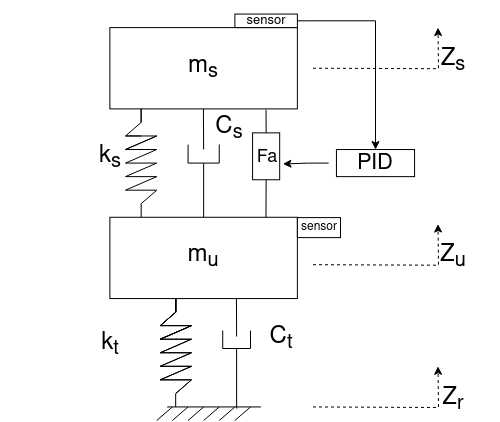
\includegraphics[width=\columnwidth]{images/qcm.png}
    \caption{Two degree of freedom quarter car model with the tire modeled as a spring and a damper.}
    \label{fig:qcm}
\end{figure}

% Newton
The differential equations for a linear model of a quarter car vehicle can be established using Newtons second law of motion and is illustrated in\:\eqref{eq:newton_sprung} and\:\eqref{eq:newton_unsprung}.
\begin{dmath}
    \label{eq:newton_sprung}
    m_s\ddot{z}_s = -k_s(z_s - z_u) - c_s(\dot{z}_s - \dot{z}_u) + F_a
\end{dmath}

\begin{equation}
    \begin{split}
        \label{eq:newton_unsprung}
        m_u\ddot{z}_u = k_s(z_s - z_u) + c_s(\dot{z}_s - \dot{z}_u) \\
        - k_t(z_u - z_r) - c_t(\dot{z}_u - \dot{z}_r) - F_a \\
        = k_s(z_s - z_u) + c_s(\dot{z}_s - \dot{z}_u) \\
        -k_t z_u - c_t\dot{z}_u + F_r - F_a
    \end{split}
\end{equation}

\begin{dmath}
    \label{eq:f_r}
    F_r = k_t z_r + c_t\dot{z}_r
\end{dmath}

% State, input and output
The state vector was defined as the sprung mass vertical displacement and velocity, as well as the unsprung mass vertical displacement and velocity, see\:\eqref{eq:state_vector}.
\begin{equation}
\label{eq:state_vector}
X = 
\begin{bmatrix}
z_s \\
\dot{z}_s \\
z_u \\
\dot{z}_u
\end{bmatrix}
\end{equation}

The input vector was defined as the force from the road and the active control force, see\:\eqref{eq:input_vector} and\:\eqref{eq:f_r}.
\begin{equation}
\label{eq:input_vector}
U = 
\begin{bmatrix}
F_r \\
F_a
\end{bmatrix}
\end{equation}

The output vector was defined as the sprung mass vertical acceleration and velocity, as well as the vertical velocity of the unsprung mass, see\:\eqref{eq:output_vector}.
\begin{equation}
\label{eq:output_vector}
Y = 
\begin{bmatrix}
\ddot{z}_s \\
\dot{z}_s \\
\dot{z}_u
\end{bmatrix}
\end{equation}

% A B C D matrices
From equations [\eqref{eq:newton_sprung},\:\eqref{eq:newton_unsprung},\:\eqref{eq:f_r},\:\eqref{eq:state_vector},\:\eqref{eq:input_vector},\:\eqref{eq:output_vector}],
\begin{comment}
With the states \eqref{eq:state_vector}, inputs \eqref{eq:input_vector}, outputs\:\eqref{eq:output_vector}\:and using\:\eqref{eq:newton_sprung}\:and\:\eqref{eq:newton_unsprung}, and substituting\:\eqref{eq:f_r}\:in\:\eqref{eq:newton_unsprung}, 
\end{comment}
the state space equations can be derived as illustrated in\:\eqref{eq:state_space}.

\begin{dmath}
\label{eq:state_space}
\left\{
\begin{array}{ll}
    \dot{X} = AX + BU \\
    Y = CX + DU
\end{array}
\right.
\end{dmath}

\begin{comment}
\begin{dmath}
    \label{eq:state_space_x}
    \dot{X} = AX + BU
\end{dmath}

\begin{dmath}
    \label{eq:state_space_y}
    Y = CX + DU
\end{dmath}
\end{comment}
The A, B, C and D matrices can then be obtained from the state space equations\:\eqref{eq:state_space} as illustrated in\:\eqref{eq:A_matrix},\:\eqref{eq:B_matrix},\:\eqref{eq:C_matrix} and\:\eqref{eq:D_matrix}.

\begin{equation}
\label{eq:A_matrix}
A = 
\begin{bmatrix}
0 & 1 & 0 & 0 \\
-\frac{k_s}{m_s} & -\frac{c_s}{m_s} & \frac{k_s}{m_s} & \frac{c_s}{m_s} \\
0 & 0 & 0 & 1 \\
\frac{k_s}{m_u} & \frac{c_s}{m_u} & \frac{-k_s-k_t}{m_u} & \frac{c_s-c_t}{m_u}
\end{bmatrix}
\end{equation}

\begin{equation}
\label{eq:B_matrix}
B = 
\begin{bmatrix}
0 & 0 \\
0 & \frac{1}{m_s} \\
0 & 0 \\
\frac{1}{m_u} & -\frac{1}{m_u}
\end{bmatrix}
\end{equation}

\begin{equation}
\label{eq:C_matrix}
C = 
\begin{bmatrix}
-\frac{k_s}{m_s} & -\frac{c_s}{m_s} & \frac{k_s}{m_s} & \frac{c_s}{m_s} \\
0 & 1 & 0 & 0 \\
0 & 0 & 0 & 1
\end{bmatrix}
\end{equation}

\begin{equation}
\label{eq:D_matrix}
D = 
\begin{bmatrix}
0 & \frac{1}{m_s} \\
0 & 0 \\
0 & 0 \\
\end{bmatrix}
\end{equation}
%-------------------------------------------------------------------------------------------------------------
\subsection{Simulation}
% Definiera olika tester för den mekatroniska simuleringen och ange tydligt syftet med varje test och varför det genomförs. Ni ska genom testerna kunna visa att systemet uppfyller de krav och mål ni ställt.

% Parameters
The parameters used for simulation of the quarter car model can be seen in Table.\:\ref{tab:parameters}. The total simulation time used was $200$ seconds. The desired vertical acceleration of the sprung mass was set to zero, $\ddot{z}_{s\_desired} = 0 \frac{\text{m}}{\text{s}^2}$.
\begin{table}[ht]
	\centering
	\begin{tabular}{|l|l|l|l|l|l|}
			\hline
			Symbol       & Value     & Unit                                         \\
			\hline
			$m_s$        & $86.5$    & $\text{kg}$                                  \\
			$m_u$        & $9.2$     & $\text{kg}$                                  \\
            $k_s$        & $4550$    & $\frac{\text{N}}{\text{m}}$                  \\
            $k_t$        & $150000$  & $\frac{\text{N}}{\text{m}}$                  \\
            $c_s$        & $300$     & $\text{N}\cdot\frac{\text{s}}{\text{m}}$     \\
            $c_t$        & $45$      & $\text{N}\cdot\frac{\text{s}}{\text{m}}$     \\
            $n$          & $0.94$    & Ratio                                        \\
			\hline
		\end{tabular}
	\caption{Parameter values used for simulation. Estimated based on\:\cite{mdhsolarteamBillMaterials}\cite{cfw16inchTypeC}.}
	\label{tab:parameters}
\end{table}

% Energy, actuator/generator control
The control between generator and actuator modes were implemented using Stateflow, see Fig.\:\ref{fig:stateflow_chart} (note that integration was done outside the Stateflow chart). The system enters actuator mode when $ (\dot{z}_s - \dot{z}_u) > 0$ which means that the sprung mass is moving faster than the unsprung mass and requires damping. The system enters generator mode when $ (\dot{z}_s - \dot{z}_u) \le 0$, and thus harvests the energy provided by the relative motion when the unsprung mass is moving faster than the sprung mass. The formula for energy consumed can be seen in\:\eqref{eq:consumed} and the energy regenerated can be seen in\:\eqref{eq:regenerated}, similar to\:\cite{yinPerformanceEvaluationActive2015}. The fraction $\frac{1}{n}$ in\:\eqref{eq:consumed} was the result of the motor efficiency in actuator mode acting on the energy consumed $n \cdot W_c$, and thus transferring it over to the right hand side results in division. In generator mode\:\eqref{eq:regenerated} it is the opposite, the motor efficiency acts on the work which drives the generator.
\begin{center}
    \begin{equation}
        \begin{split}
            \label{eq:consumed}
            W_c = \int_{0}^{t} \frac{F_a}{n} \cdot (\dot{z}_s - \dot{z}_u), \: F_a \cdot (\dot{z}_s - \dot{z}_u) \le 0
        \end{split}
    \end{equation}
\end{center}
\begin{center}
    \begin{equation}
        \begin{split}
            \label{eq:regenerated}
            W_r = \int_{0}^{t} n \cdot F_a \cdot (\dot{z}_s - \dot{z}_u), \: F_a \cdot (\dot{z}_s - \dot{z}_u) \ge 0
        \end{split}
    \end{equation}
\end{center}
The total energy gained or consumed by the actuator was then calculated by\:\eqref{eq:actuator_energy}.
\begin{equation}
    \label{eq:actuator_energy}
    W_{total} = W_c + W_r
\end{equation}
\begin{figure}
    \centering
    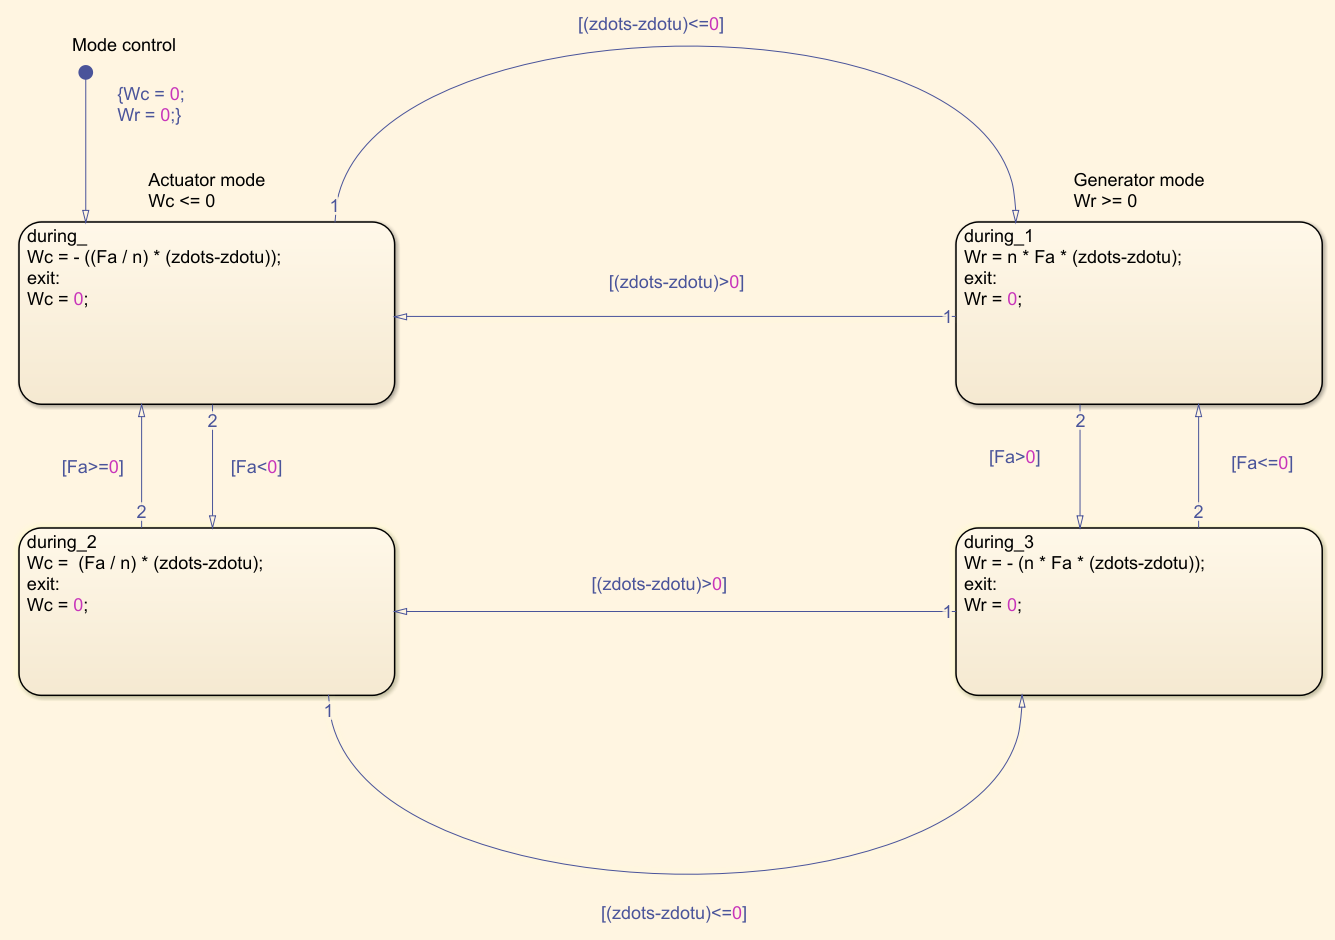
\includegraphics[width = \columnwidth]{images/stateflow_chart.png}
    \caption{The Stateflow chart which controls the switching between generator and actuator modes. Note that the integration part of the equation for energy consumed and regenerated was done outside the Stateflow chart.}
    \label{fig:stateflow_chart}
\end{figure}
The self supplying efficiency, $n_{ss}$, was defined as the fraction of energy regenerated to energy consumed, see\:\eqref{eq:self_supplying_efficiency}.
\begin{dmath}
    \label{eq:self_supplying_efficiency}
    n_{ss} = \frac{|W_r|}{|W_c|}
\end{dmath}

% PID
A PID controller was used to minimize the error which was the deviation of actual value from the setpoint. The setpoint was the desired vertical acceleration of the sprung mass $\ddot{z}_{s\_desired} = 0\frac{\text{m}}{\text{s}^2}$. The actual value was the first component of the output vector, $\ddot{z}_s$, this was provided by the negative feedback. See Fig.\:\ref{fig:simulink_diagram} for the complete simulation block diagram in Simulink (note that the time dependency of variables has been excluded to help minimize cluttering). The final PID controller values were: $P = 500$, $I = 5$, $D = 1$, taken from\:\cite{liuModelingSimulationEnergyRegenerative2019}.
\begin{figure}
    \centering
    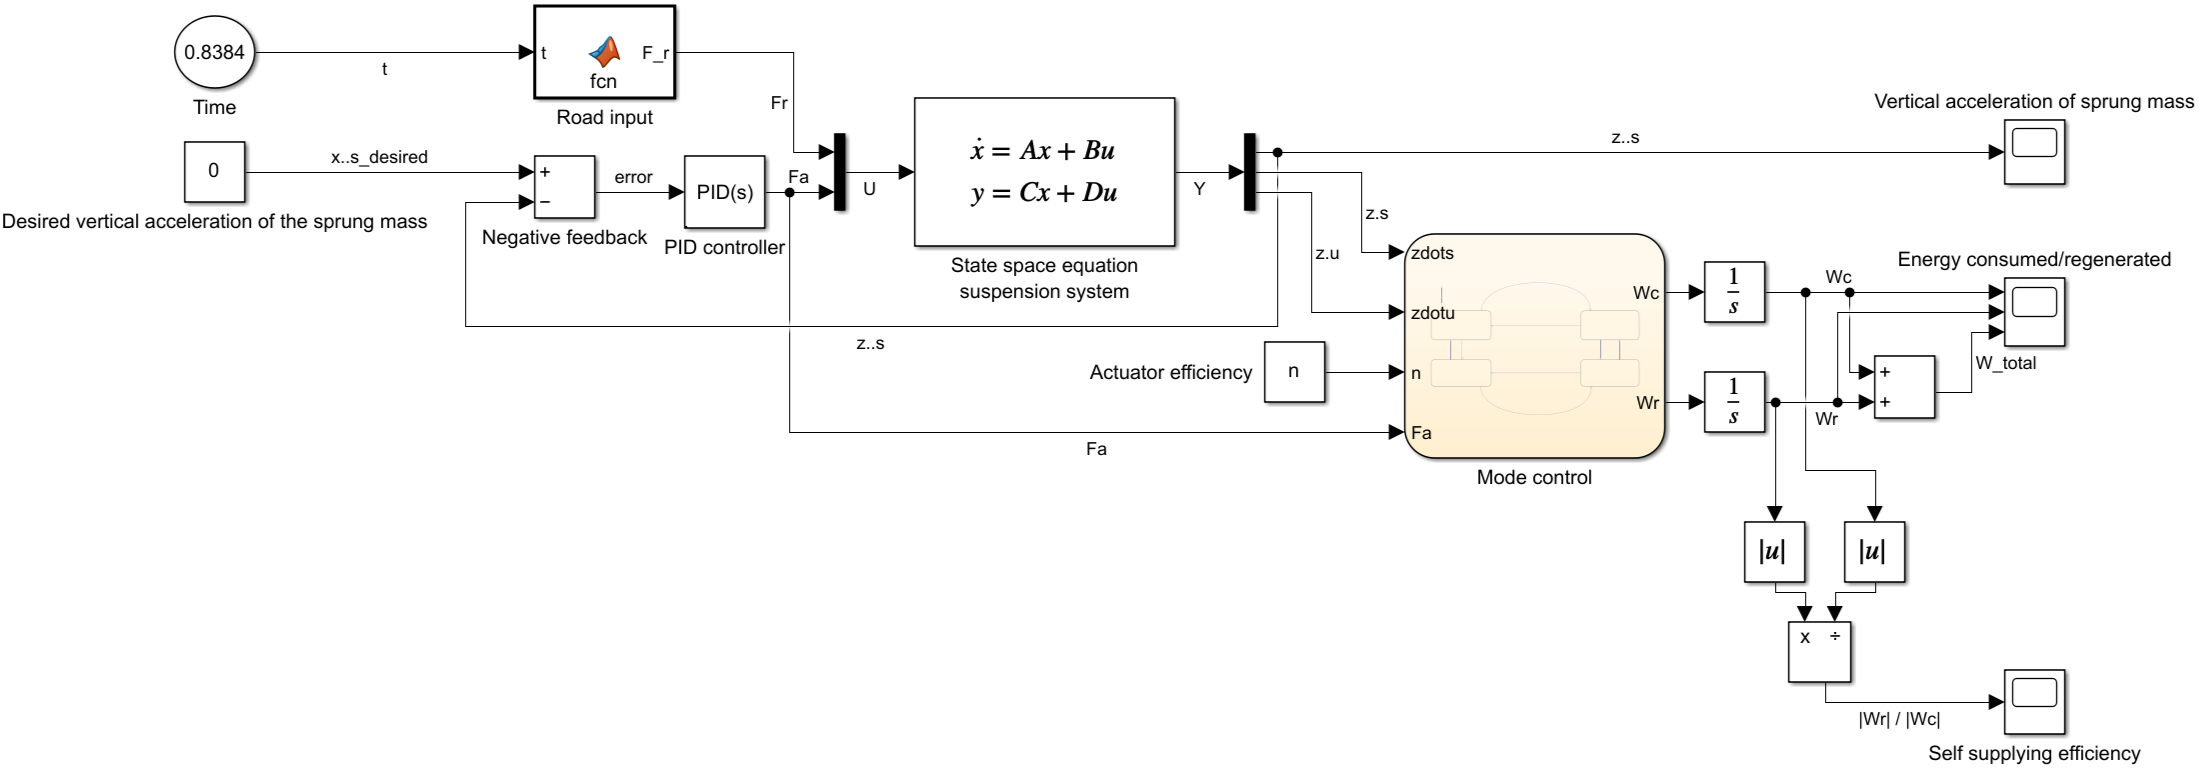
\includegraphics[width=\columnwidth]{images/simulink_diagram.png}
    \caption{The complete block diagram in Simulink. Note that the time dependency of variables has been excluded to help minimize cluttering.}
    \label{fig:simulink_diagram}
\end{figure}

% Tests
For the tests, a random road model was created, which consisted of applying different types of noise (random road input) to the road input to simulate different types of road conditions and speeds. The random road model can be seen in\:\eqref{eq:noise}.
\begin{dmath}
    \label{eq:noise}
    F_r = | a_1 \cdot sin(f_1 \cdot t + p_1) + a_2 \cdot cos(f_2 \cdot t + p_2) |
\end{dmath}
The tests were performed with the purpose of verifying the system and ensuring road comfort was maintained and evaluating the system based on the performance metrics. The different tests can be seen in Table.\:\ref{tab:tests}. It should be noted that the test names are not absolute, a test which was named as a certain speed can also be considered as a lower speed but worse road condition.
\begin{table}[ht]
	\centering
	\resizebox{\columnwidth}{!}{\noindent\begin{tabular}{|l|l|l|l|l|l|l|l|}
			\hline
			Test                                     & $t$ (s)           & $a_1$ (N)     & $f_1$ (Hz)    & $p_1$ (rad)    & $a_2$ (N)        & $f_2$ (Hz)     & $p_2$ (Rad)      \\
			\hline
			Speed bump                               & 10, 40, 80, 90    & 0             & 0             & 0              & [200000 400000]  & 0              & 0                \\
			$0-10\frac{\text{km}}{\text{h}}$         & [0 10)            & [0 1000]      & [0 2]         & [0 1]          & [0 1000]         & [0 2]          & [0 1]            \\
            $10-20\frac{\text{km}}{\text{h}}$        & (10 20)           & [0 4000]      & [1 3]         & [0 1]          & [0 4000]         & [1 3]          & [0 1]            \\
            $20-30\frac{\text{km}}{\text{h}}$        & (20 30)           & [0 6000]      & [3 5]         & [0 1]          & [0 6000]         & [3 5]          & [0 1]            \\
            $30-40\frac{\text{km}}{\text{h}}$        & (30 40)           & [0 9000]      & [4 6]         & [0 1]          & [0 9000]         & [4 6]          & [0 1]            \\
            $40-50\frac{\text{km}}{\text{h}}$        & (40 50)           & [0 11000]     & [6 8]         & [0 1]          & [0 11000]        & [6 8]          & [0 1]            \\
            $50-60\frac{\text{km}}{\text{h}}$        & (50 60)           & [0 13000]     & [7 9]         & [0 1]          & [0 13000]        & [7 9]          & [0 1]            \\
            $60-70\frac{\text{km}}{\text{h}}$        & (60 70)           & [0 16000]     & [9 11]        & [0 1]          & [0 16000]        & [9 11]         & [0 1]            \\
            $70-80\frac{\text{km}}{\text{h}}$        & (70 80)           & [0 18000]     & [10 12]       & [0 1]          & [0 18000]        & [10 12]        & [0 1]            \\
            $80-90\frac{\text{km}}{\text{h}}$        & (80 90)           & [0 21000]     & [12 14]       & [0 1]          & [0 21000]        & [12 14]        & [0 1]            \\
            $90-100\frac{\text{km}}{\text{h}}$       & (90 100)          & [0 23000]     & [14 16]       & [0 1]          & [0 23000]        & [14 16]        & [0 1]            \\
            $100-110\frac{\text{km}}{\text{h}}$      & (100 150)         & [0 26000]     & [15 17]       & [0 1]          & [0 26000]        & [15 17]        & [0 1]            \\
            Rest                                     & (150 $\infty$)      & 0             & 0             & 0              & 0                & 0              & 0                \\
			\hline
		\end{tabular}}
	\caption{Description of all the tests for the system. Test names can also be considered as a lower speed but worse road condition.}
	\label{tab:tests}
\end{table}

%-------------------------------------------------------------------------------------------------------------
\subsection{Design}
% Konstruera en teoretisk systemdesign och motivera den med hänsyn till resultaten från modellen och simuleringen.
A theoretical system design for the proposed RASS model was created. Important considerations for its viability and integration with the MDH solar car were also covered. Unfortunately, because of the insufficient documentation of the MDH solar car, an actual theoretical system design was not relevant since it would require to many assumptions. Therefor this section describes considerations for a theoretical system design if proper information was available.
\subsubsection{Sensors}
The proposed system requires two types of sensors: accelerometers and velocity sensors.
An accelerometer is necessary for monitoring the vertical acceleration of the sprung mass, which is used by the active suspension control. Dual accelerometers (redundancy) would be placed in each wheelhouse as close to the wheel as possible.

The use of a pair of velocity sensors, dual sensors in the wheel and dual sensors in the wheelhouse (redundancy), for each wheel of the car is necessary for mode control and calculating the energy regenerated and consumed by the RASS, see\:\eqref{eq:consumed} and\:\eqref{eq:regenerated}.
Both the accelerometers and velocity sensors must be resistant to vibration, liquid and smaller impacts from objects like gravel. Possible accelerometer options include MEMS or piezoelectric sensors. Some velocity sensors which might work well include hall effect sensors or piezoelectric velocity sensors.
However the final choice of sensors must be done after substantial testing, once proper functioning with the rest of the system and electrical network has been ensured, as well as final cost considerations.

\subsubsection{Actuator and generator}
The use of a DC motor as the actuator for a RASS is common and it can function as both actuator and generator\:\cite{liuTransmissionEnergyharvestingStudy2021}\cite{liuModelingSimulationEnergyRegenerative2019}\cite{zhengNovelEnergyregenerativeActive2008}. The choice of a DC motor thus serves as a good outset option for the initial theoretical system design. 
Brushless DC motors are common options\:\cite{zhengNovelEnergyregenerativeActive2008}, especially permanent magnet brushless DC motors\:\cite{liuTransmissionEnergyharvestingStudy2021}\cite{liuModelingSimulationEnergyRegenerative2019}\cite{yongchaozhangExperimentalVerificationEnergyregenerative2007}, a permanent magnet brushless DC motor was therefor chosen. 
One actuator/generator is required for each wheel, and thus one motor for each wheel. This will result in significant cost and power requirements. Thus the final choice of motor must consider even more so the energy consumption characteristics of the motor as well as the cost, along with other important considerations like torque and its ability to be integrated with the control electronics and the feedback system.
The final choice of permanent magnet brushless DC motor is thus very complex since it must integrate well with the existing electronics and systems of the MDU solar car.

\subsubsection{Control systems}
A number of control systems are necessary for the RASS to function, including: mode control, active suspension control and energy control. All control units would be implemented as dual units because of redundancy. 
The mode control uses the velocity sensor values and is necessary to switch between the actuator mode and generator mode since both can not be used at the same time. One mode control unit is required for each actuator, the mode control was implemented as a Stateflow chart in the simulations. The mode control unit would most likely be an embedded system with a real-time operating system (RTOS).
The active suspension control uses the accelerometer values to regulate the active control force to minimize sprung mass vertical acceleration. The active suspension control was implemented as a PID controller in the Simulink simulations. One active suspension control unit is required per wheelhouse. The active suspension control unit would much like the mode control unit most likely be implemented as an embedded system using a RTOS.
The power management and battery management systems and controllers need to be expanded to allow for the regenerative part of the RASS system to function and be integrated. Proper management of the energy harvested and how it should be stored, optimization of energy regeneration and power delivery to the actuator are some of the important aspects related to the different management systems.

\subsubsection{Energy storage}
The use of capacitors or ultra capacitors could improve energy regeneration and provide more optimal utilization of the energy harvested from the RASS, much like it does for regenerative braking (see Introduction\:\ref{section:intro}), but would increase the initial cost of the system. However for this initial theoretical system design, this was skipped for simplicity, and all energy storage needs would be handled by the batteries.

%batteries?

\subsubsection{Power electronics}
The RASS requires converters for converting the electricity from storage to actuator and from generator to storage.
For storage to actuator this would roughly be a DC-DC converter from $126\:\text{V}$\:\cite{mdhsolarteamBillMaterials} to $12-48\:\text{V}$ (depending on motor and the required output torque).
Also, the generated energy needs to be stepped up by a DC-DC converter to be able to be stored in the $126\:\text{V}$ battery\:\cite{mdhsolarteamBillMaterials}.

\subsubsection{Integration}
Integrating the RASS with the MDH solar car requires several considerations. One such consideration is the mass distribution, this is especially important since the MDH solar car uses in-wheel drive and thus a lot of the mass is unsprung mass. A low unsprung mass would mean less force is transmitted to the sprung mass increasing ride comfort. As mentioned previously, the model assumes all wheels have equal mass and are identical, this is however not the case in reality, the rear wheels have significantly more mass because of in-wheel configuration in only the rear wheels. Therefor, a proper model should be implemented covering all four wheels of the car taking the differences in mass into account. The majority of the mass of the RASS should also be attempted to be anchored in the sprung mass, for example the heavier side of the damper, to prevent increasing unsprung mass.
Integrating the RASS into the current electrical network and the current suspension system of the car is also tricky.
Considerations such as whether sufficient power can be provided to the RASS given the current electrical network, additional load and possible impact on the performance given increased power demands and possible electromagnetic compatibility (EMC) issues.
Considerations regarding integrating the RASS with the current suspension system was not possible because of the insufficient documentation of the current suspension system. However, possible considerations include space and changes of the passive springs and dampers.

\subsubsection{Safety}
Redundancy would be used to ensure the system does not stop functioning or become unsafe if a part of the RASS stops being operational. This includes: dual sensors, dual communications channels, dual control units, redundant feedback systems, springs and actuators with redundancy if one fails, additional or emergency power supply if main power supply fails, multiple algorithms and using voting between them.
The proposed theoretical system requires significant testing to ensure it meets its functional requirements and is safe.

\subsubsection{User interface}
A user interface to allow proper view of the system status and user control of the system. A user interface would in turn require a controller and would probably be implemented using a design pattern like model view presenter (MVP) and running a RTOS.

\subsubsection{Performance tuning}
The control algorithms would require performance tuning to function optimally. This would include global optimization and real time optimization\:\cite{carlenerikssonEVHEVFramdrivning2023}. Updates to the control algorithms is also necessary to consider in case of faults and improvements.

\subsubsection{Regulatory compliance}
Regulations and standards for suspension systems were unavailable because of the cost of access to such documents. However it is paramount that such standards are followed and the regulations obeyed.

\subsubsection{Mass}
As previously noted, the system design must not cause mass distribution problems nor increase the vehicles mass above a certain limit. This could not be assessed since information regarding mass was not available.
%This is not expected to be a problem for the proposed RASS. 

\subsubsection{Dimension}
The system must also have viable dimensions to fit the MDH solar car. This could not be established properly since proper information was not available.

\subsubsection{Cost}
The cost of the system is one of the most important aspects, however, since no budget was available, this could not be evaluated.



%-------------------------------------------------------------------------------------------------------------
% Översätt den valda designen till eventuella arbetsritningar, kretsscheman, etc.
% Ritningar och en materialförteckning (BoM) för systemet med en tydlig motivering
% CAD?

A flowchart describing the theoretical system design and the workings of the model can be seen in Fig.\:\ref{fig:RASS_flowchart}. The user interface and some other interactions were excluded from the flowchart shown in Fig.\:\ref{fig:RASS_flowchart}, because the focus was on the suspension part of the system.

\begin{figure}
    \centering
    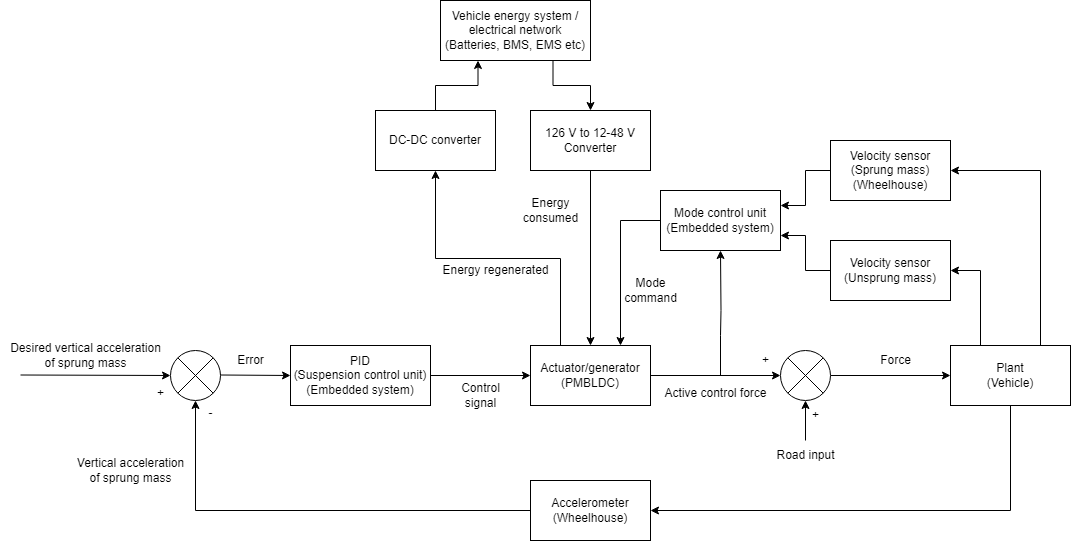
\includegraphics[width=\columnwidth]{images/RASS_flowchart.png}
    \caption{RASS flowchart describing the theoretical system design and its functionality. Note that some interactions and the user interface has been excluded since the focus was on the suspension part of the system.}
    \label{fig:RASS_flowchart}
\end{figure}

%-------------------------------------------------------------------------------------------------------------